\documentclass[aspectratio=169]{beamer}

\usetheme{default}
\usecolortheme{default}
\usefonttheme{professionalfonts}

\usepackage[T1]{fontenc}
\usepackage{lmodern}
\usepackage{tikz}
\usepackage{booktabs}
\usepackage{array}
\usepackage{tabularx}
\usepackage{graphicx}
\usetikzlibrary{positioning,arrows.meta,calc,fit,shapes.geometric}

\definecolor{MemphisBlue}{RGB}{26,62,122}
\definecolor{LightBand}{RGB}{244,247,252}
\definecolor{MidBand}{RGB}{229,236,247}
\definecolor{SoftGray}{RGB}{90,96,108}
\definecolor{AccentGreen}{RGB}{61,130,89}
\definecolor{AccentOrange}{RGB}{194,111,46}
\definecolor{AccentRed}{RGB}{168,65,65}

\setbeamertemplate{navigation symbols}{}
\setbeamertemplate{itemize item}{\color{MemphisBlue}$\blacktriangleright$}
\setbeamertemplate{itemize subitem}{\color{MemphisBlue}$\circ$}
\setbeamercolor{title}{fg=MemphisBlue}
\setbeamercolor{frametitle}{fg=MemphisBlue,bg=white}
\setbeamercolor{author in head/foot}{fg=MemphisBlue,bg=white}
\setbeamercolor{date in head/foot}{fg=MemphisBlue,bg=white}
\setbeamercolor{block body}{bg=LightBand,fg=black}
\setbeamerfont{frametitle}{size=\Large,series=\bfseries}
\setbeamerfont{title}{size=\LARGE,series=\bfseries}
\setbeamerfont{subtitle}{size=\large}
\setbeamerfont{normal text}{size=\normalsize}

\setbeamertemplate{footline}{%
  \leavevmode%
  \hbox{%
    \begin{beamercolorbox}[wd=.76\paperwidth,ht=2.6ex,dp=1.2ex,leftskip=1.2em]{author in head/foot}%
      \scriptsize NDNSF-UAV-APP: Design and Mechanisms
    \end{beamercolorbox}%
    \begin{beamercolorbox}[wd=.24\paperwidth,ht=2.6ex,dp=1.2ex,rightskip=1.2em plus1fil]{date in head/foot}%
      \scriptsize \insertframenumber/\inserttotalframenumber
    \end{beamercolorbox}%
  }%
}

\newcommand{\bluebox}[1]{%
  \begin{beamercolorbox}[rounded=true,shadow=false,sep=0.65em,wd=0.94\linewidth]{block body}
  #1
  \end{beamercolorbox}
}

\newcommand{\evidence}[1]{%
  \vfill\par\noindent
  \begin{minipage}{\linewidth}
  \raggedright{\color{SoftGray}\tiny Evidence: #1}\par
  \end{minipage}
}

\newcolumntype{Y}{>{\raggedright\arraybackslash}X}

\tikzset{
  flow/.style={-{Stealth[length=2.2mm]},thick,draw=MemphisBlue},
  backflow/.style={{Stealth[length=2.2mm]}-,thick,draw=MemphisBlue},
  dashflow/.style={-{Stealth[length=2.2mm]},thick,dashed,draw=AccentOrange},
  thinflow/.style={-{Stealth[length=1.8mm]},semithick,draw=MemphisBlue},
  box/.style={draw=MemphisBlue,fill=LightBand,rounded corners=2pt,
    minimum height=0.72cm,align=center,font=\scriptsize},
  strongbox/.style={draw=MemphisBlue,fill=MidBand,rounded corners=2pt,
    minimum height=0.78cm,align=center,font=\scriptsize\bfseries},
  greenbox/.style={draw=AccentGreen,fill=AccentGreen!10,rounded corners=2pt,
    minimum height=0.72cm,align=center,font=\scriptsize},
  orangebox/.style={draw=AccentOrange,fill=AccentOrange!10,rounded corners=2pt,
    minimum height=0.72cm,align=center,font=\scriptsize},
  redbox/.style={draw=AccentRed,fill=AccentRed!8,rounded corners=2pt,
    minimum height=0.72cm,align=center,font=\scriptsize}
}

\title{NDNSF-UAV-APP}
\subtitle{Named Services for Secure Control, Adaptive Video, and Multi-Drone Operations}
\author{Tianxing Ma}
\institute{Department of Computer Science\\University of Memphis}
\date{July 2026}

\begin{document}

\begin{frame}[plain]
  \titlepage
\end{frame}

\begin{frame}{Why an NDN-Native UAV Application?}
\footnotesize
\begin{columns}[T]
\begin{column}{0.48\textwidth}
\textbf{One mission combines different communication needs}
\begin{itemize}
  \item Safety-sensitive commands need authorization and prompt failure.
  \item Telemetry and readiness must stay tied to the selected vehicle.
  \item Live video is continuous; recordings and logs are durable objects.
  \item Multiple mobile drones may be busy, disconnected, or replaceable.
\end{itemize}
\end{column}
\begin{column}{0.48\textwidth}
\begin{center}
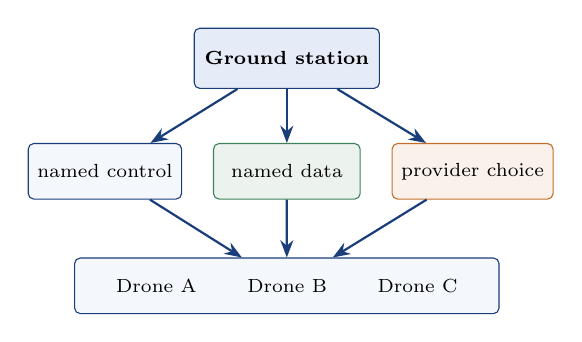
\begin{tikzpicture}[node distance=0.45cm,scale=0.98,transform shape]
  \node[strongbox,minimum width=2.4cm] (gs) {Ground station};
  \node[box,below left=0.7cm and 0.15cm of gs,minimum width=1.9cm] (control) {named control};
  \node[greenbox,below=0.7cm of gs,minimum width=1.9cm] (data) {named data};
  \node[orangebox,below right=0.7cm and 0.15cm of gs,minimum width=1.9cm] (select) {provider choice};
  \node[box,below=0.75cm of data,minimum width=5.5cm] (drones) {Drone A \qquad Drone B \qquad Drone C};
  \draw[flow] (gs) -- (control);
  \draw[flow] (gs) -- (data);
  \draw[flow] (gs) -- (select);
  \draw[flow] (control) -- (drones);
  \draw[flow] (data) -- (drones);
  \draw[flow] (select) -- (drones);
\end{tikzpicture}
\end{center}
\end{column}
\end{columns}

\vspace{0.4em}
\bluebox{The application binds UAV operations to \textbf{service and data names}, not to one fixed endpoint connection.}
\evidence{NDNSF-UAV-APP/README.md: Why This Application Exists}
\end{frame}

\begin{frame}{Responsibility Boundary}
\footnotesize
\begin{center}
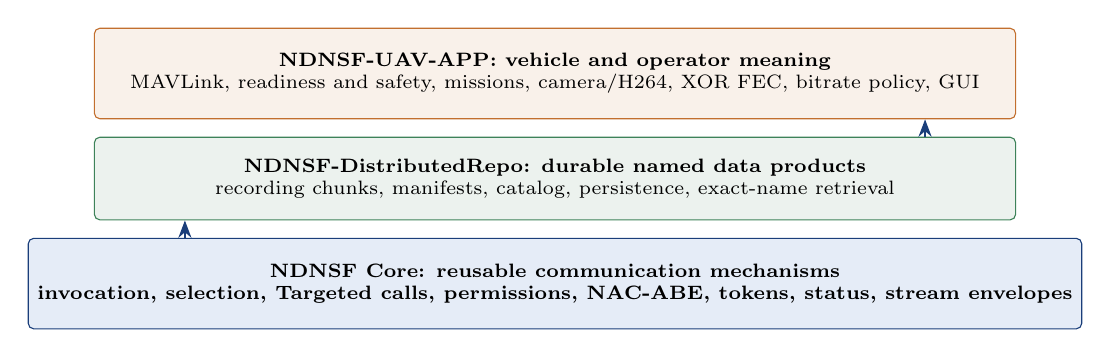
\begin{tikzpicture}[node distance=0.3cm]
  \node[orangebox,minimum width=11.7cm,minimum height=1.15cm] (app) {
    \textbf{NDNSF-UAV-APP: vehicle and operator meaning}\\
    MAVLink, readiness and safety, missions, camera/H264, XOR FEC, bitrate policy, GUI
  };
  \node[greenbox,below=0.22cm of app,minimum width=11.7cm,minimum height=1.05cm] (repo) {
    \textbf{NDNSF-DistributedRepo: durable named data products}\\
    recording chunks, manifests, catalog, persistence, exact-name retrieval
  };
  \node[strongbox,below=0.22cm of repo,minimum width=11.7cm,minimum height=1.15cm] (core) {
    \textbf{NDNSF Core: reusable communication mechanisms}\\
    invocation, selection, Targeted calls, permissions, NAC-ABE, tokens, status, stream envelopes
  };
  \draw[flow] ([xshift=-4.7cm]core.north) -- ([xshift=-4.7cm]repo.south);
  \draw[flow] ([xshift=4.7cm]repo.north) -- ([xshift=4.7cm]app.south);
\end{tikzpicture}
\end{center}

\vspace{0.25em}
\bluebox{Core provides generic envelopes and security; the UAV application remains responsible for flight semantics and policy.}
\evidence{docs/ndnsf-core-app-boundary.md; specs/070-uav-qgc-parity-boundary}
\end{frame}

\begin{frame}{Three Runtime Roles}
\footnotesize
\begin{center}
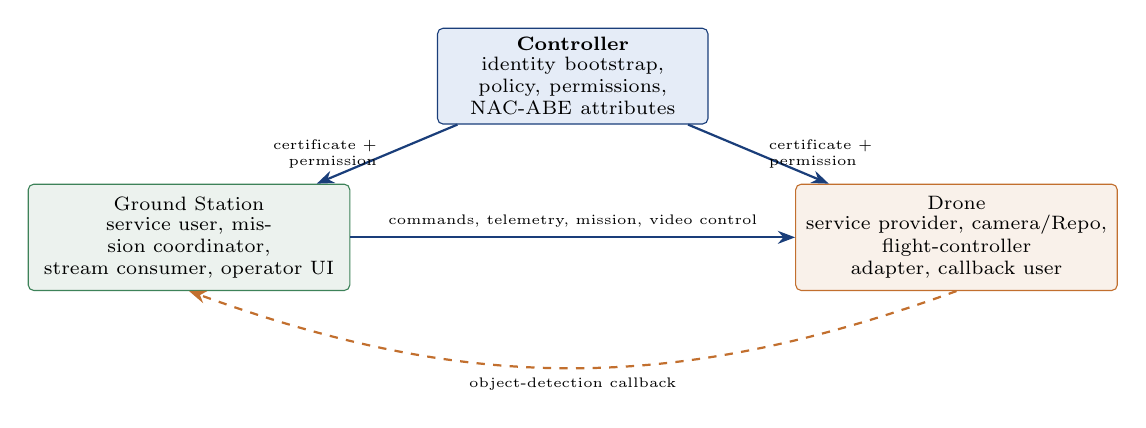
\begin{tikzpicture}[node distance=0.55cm]
  \node[strongbox,text width=3.2cm,minimum height=1.15cm] (controller) {
    Controller\\[-0.1em]
    \normalfont identity bootstrap, policy, permissions, NAC-ABE attributes
  };
  \node[greenbox,below left=0.75cm and 1.1cm of controller,text width=3.85cm,minimum height=1.35cm] (gs) {
    Ground Station\\[-0.1em]
    \normalfont service user, mission coordinator,\\stream consumer, operator UI
  };
  \node[orangebox,below right=0.75cm and 1.1cm of controller,text width=3.85cm,minimum height=1.35cm] (drone) {
    Drone\\[-0.1em]
    \normalfont service provider, camera/Repo,\\flight-controller adapter, callback user
  };
  \draw[flow] (controller) -- node[left,font=\tiny,align=right] {certificate +\\permission} (gs);
  \draw[flow] (controller) -- node[right,font=\tiny,align=left] {certificate +\\permission} (drone);
  \draw[flow] (gs) -- node[above,font=\tiny] {commands, telemetry, mission, video control} (drone);
  \draw[dashflow] (drone.south) to[bend left=20] node[below,font=\tiny] {object-detection callback} (gs.south);
\end{tikzpicture}
\end{center}

\vspace{0.35em}
\begin{columns}[T]
\begin{column}{0.48\textwidth}
\textbf{Typical PC}: Controller + Ground Station + NFD
\end{column}
\begin{column}{0.48\textwidth}
\textbf{Each vehicle}: DroneAPP + NFD + camera + MAVLink link
\end{column}
\end{columns}
\evidence{UavDroneApp.cpp; UavGroundStationApp.cpp; README deployment section}
\end{frame}

\begin{frame}{Service Containers, Not One Monolithic RPC}
\footnotesize
\begin{columns}[T]
\begin{column}{0.49\textwidth}
\begin{center}
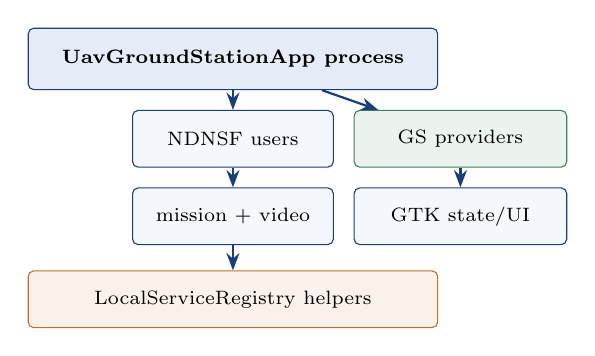
\begin{tikzpicture}[node distance=0.25cm]
  \node[strongbox,minimum width=5.2cm] (gsprocess) {UavGroundStationApp process};
  \node[box,below=of gsprocess,minimum width=2.55cm] (users) {NDNSF users};
  \node[greenbox,right=0.25cm of users,minimum width=2.7cm] (gsprovider) {GS providers};
  \node[box,below=of users,minimum width=2.55cm] (workflow) {mission + video};
  \node[box,right=0.25cm of workflow,minimum width=2.7cm] (gui) {GTK state/UI};
  \node[orangebox,below=0.32cm of workflow,minimum width=5.2cm] (gslocal) {LocalServiceRegistry helpers};
  \draw[flow] (gsprocess) -- (users);
  \draw[flow] (gsprocess) -- (gsprovider);
  \draw[flow] (users) -- (workflow);
  \draw[flow] (gsprovider) -- (gui);
  \draw[flow] (workflow) -- (gslocal);
\end{tikzpicture}
\end{center}
\end{column}
\begin{column}{0.49\textwidth}
\begin{center}
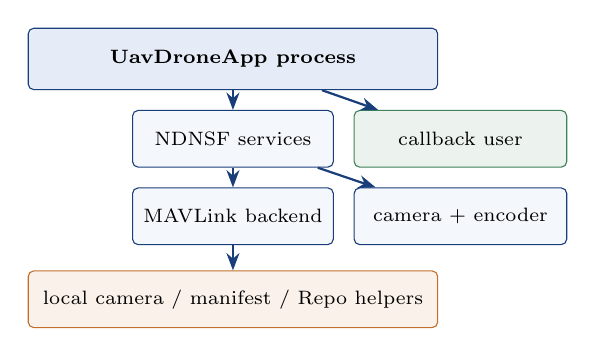
\begin{tikzpicture}[node distance=0.25cm]
  \node[strongbox,minimum width=5.2cm] (droneprocess) {UavDroneApp process};
  \node[box,below=of droneprocess,minimum width=2.55cm] (providers) {NDNSF services};
  \node[greenbox,right=0.25cm of providers,minimum width=2.7cm] (callback) {callback user};
  \node[box,below=of providers,minimum width=2.55cm] (mav) {MAVLink backend};
  \node[box,right=0.25cm of mav,minimum width=2.7cm] (camera) {camera + encoder};
  \node[orangebox,below=0.32cm of mav,minimum width=5.2cm] (local) {local camera / manifest / Repo helpers};
  \draw[flow] (droneprocess) -- (providers);
  \draw[flow] (droneprocess) -- (callback);
  \draw[flow] (providers) -- (mav);
  \draw[flow] (providers) -- (camera);
  \draw[flow] (mav) -- (local);
\end{tikzpicture}
\end{center}
\end{column}
\end{columns}

\vspace{0.35em}
\bluebox{One process shares identity, configuration, hardware, and lifecycle; every remote service remains separately named and permission-controlled.}
\evidence{DroneServiceContainer.inc.hpp; GroundStationServiceContainer.inc.hpp}
\end{frame}

\begin{frame}{Named Services and Invocation Modes}
\scriptsize
\renewcommand{\arraystretch}{1.12}
\begin{tabularx}{\textwidth}{>{\ttfamily}p{4.6cm} p{2.7cm} Y}
\toprule
\textbf{Name} & \textbf{Mode} & \textbf{Purpose} \\
\midrule
/UAV/MAVLink/Execute & Targeted only & known-drone low-latency command path \\
/UAV/Telemetry/GetStatus & normal +\newline Targeted & discovery or selected-drone state refresh \\
/UAV/Mission/Assign & normal & multi-provider mission-slot selection \\
/<drone>/UAV/Camera/Video & normal & provider-specific Start/Stop control \\
/<drone>/UAV/MAVLink/\newline Parameters & normal & vehicle capability and parameter snapshot \\
/<drone>/UAV/Preflight/\newline Checklist & normal & typed operator readiness details \\
/<drone>/UAV/Camera/\newline Recording/Manifest & normal & discover durable recording chunks \\
/UAV/GS/ObjectDetection & normal & drone-to-ground-station compute callback \\
\bottomrule
\end{tabularx}

\vspace{0.35em}
\bluebox{Shared service names allow provider selection; provider-specific names address one physical vehicle or its data product.}
\evidence{shared/UavNames.hpp; DroneServiceContainer::installServiceInstances}
\end{frame}

\begin{frame}{Secure Startup and Invocation}
\footnotesize
\begin{center}
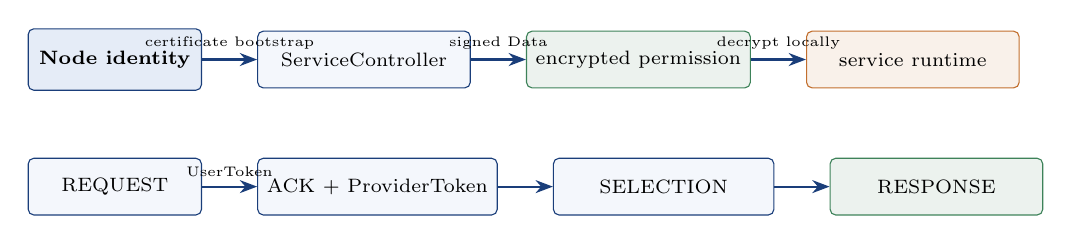
\begin{tikzpicture}[node distance=0.55cm]
  \node[strongbox,minimum width=2.2cm] (identity) {Node identity};
  \node[box,right=0.7cm of identity,minimum width=2.7cm] (controller) {ServiceController};
  \node[greenbox,right=0.7cm of controller,minimum width=2.8cm] (permission) {encrypted permission};
  \node[orangebox,right=0.7cm of permission,minimum width=2.7cm] (runtime) {service runtime};
  \draw[flow] (identity) -- node[above,font=\tiny] {certificate bootstrap} (controller);
  \draw[flow] (controller) -- node[above,font=\tiny] {signed Data} (permission);
  \draw[flow] (permission) -- node[above,font=\tiny] {decrypt locally} (runtime);

  \node[box,below=0.85cm of identity,minimum width=2.2cm] (req) {REQUEST};
  \node[box,right=0.7cm of req,minimum width=2.7cm] (ack) {ACK + ProviderToken};
  \node[box,right=0.7cm of ack,minimum width=2.8cm] (sel) {SELECTION};
  \node[greenbox,right=0.7cm of sel,minimum width=2.7cm] (resp) {RESPONSE};
  \draw[flow] (req) -- node[above,font=\tiny] {UserToken} (ack);
  \draw[flow] (ack) -- (sel);
  \draw[flow] (sel) -- (resp);
\end{tikzpicture}
\end{center}

\vspace{0.55em}
\begin{itemize}
  \item REQUEST/SELECTION use service attributes; ACK/RESPONSE use permission attributes.
  \item One-time user/provider tokens bind the handshake and reject replay.
  \item Controller permission Data is signed and encrypted to the target identity certificate.
\end{itemize}
\evidence{ServiceController; ServiceUser/ServiceProvider security path; UAV deployment README}
\end{frame}

\begin{frame}{Targeted MAVLink Command Path}
\footnotesize
\begin{center}
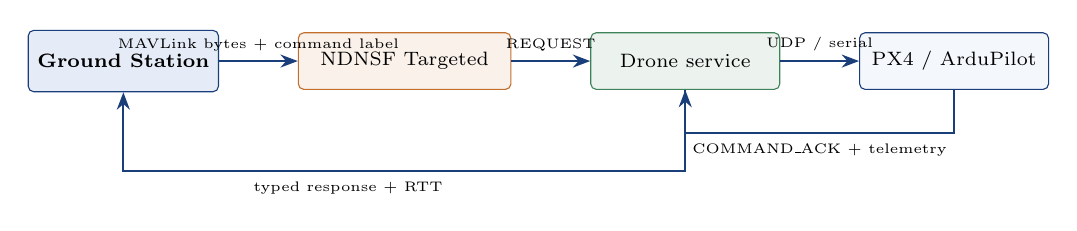
\begin{tikzpicture}[node distance=0.65cm]
  \node[strongbox,minimum width=2.4cm] (gs) {Ground Station};
  \node[orangebox,right=1.0cm of gs,minimum width=2.7cm] (ndnsf) {NDNSF Targeted};
  \node[greenbox,right=1.0cm of ndnsf,minimum width=2.4cm] (drone) {Drone service};
  \node[box,right=1.0cm of drone,minimum width=2.4cm] (fc) {PX4 / ArduPilot};
  \draw[flow] (gs) -- node[above,font=\tiny] {MAVLink bytes + command label} (ndnsf);
  \draw[flow] (ndnsf) -- node[above,font=\tiny] {REQUEST} (drone);
  \draw[flow] (drone) -- node[above,font=\tiny] {UDP / serial} (fc);
  \draw[backflow] (drone.south) -- ++(0,-0.55cm) -| node[below,pos=0.25,font=\tiny] {COMMAND\_ACK + telemetry} (fc.south);
  \draw[backflow] (gs.south) -- ++(0,-1.0cm) -| node[below,pos=0.2,font=\tiny] {typed response + RTT} (drone.south);
\end{tikzpicture}
\end{center}

\vspace{0.55em}
\begin{columns}[T]
\begin{column}{0.48\textwidth}
\textbf{First use}
\begin{itemize}
  \item authenticated ACK/selection bootstrap
  \item obtain a batch of one-time token pairs
\end{itemize}
\end{column}
\begin{column}{0.48\textwidth}
\textbf{Later commands}
\begin{itemize}
  \item request/response-only Targeted calls
  \item permissions, token checks, and replay protection remain
\end{itemize}
\end{column}
\end{columns}
\evidence{sendMavlinkCommandToDrone; ServiceProvider TargetedOnly registration}
\end{frame}

\begin{frame}{Typed State Drives the Operator Workflow}
\footnotesize
\begin{columns}[T]
\begin{column}{0.56\textwidth}
\begin{center}
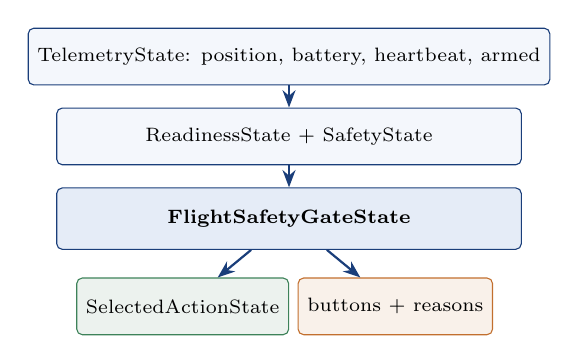
\begin{tikzpicture}[node distance=0.28cm]
  \node[box,minimum width=5.9cm] (telemetry) {TelemetryState: position, battery, heartbeat, armed};
  \node[box,below=of telemetry,minimum width=5.9cm] (readiness) {ReadinessState + SafetyState};
  \node[strongbox,below=of readiness,minimum width=5.9cm] (gate) {FlightSafetyGateState};
  \node[greenbox,below=0.35cm of gate,xshift=-1.35cm,minimum width=2.4cm] (actions) {SelectedActionState};
  \node[orangebox,below=0.35cm of gate,xshift=1.35cm,minimum width=2.4cm] (ui) {buttons + reasons};
  \draw[flow] (telemetry) -- (readiness);
  \draw[flow] (readiness) -- (gate);
  \draw[flow] (gate) -- (actions);
  \draw[flow] (gate) -- (ui);
\end{tikzpicture}
\end{center}
\end{column}
\begin{column}{0.41\textwidth}
\textbf{Command lifecycle}
\begin{center}
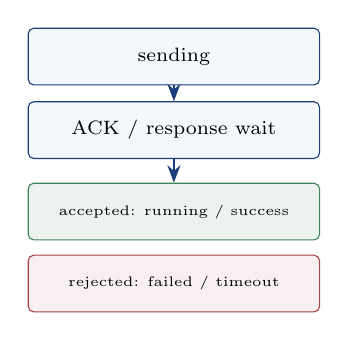
\begin{tikzpicture}[node distance=0.2cm]
  \node[box,minimum width=3.7cm] (send) {sending};
  \node[box,below=of send,minimum width=3.7cm] (wait) {ACK / response wait};
  \node[greenbox,below=0.3cm of wait,minimum width=3.7cm,font=\tiny] (ok) {accepted: running / success};
  \node[redbox,below=0.18cm of ok,minimum width=3.7cm,font=\tiny] (bad) {rejected: failed / timeout};
  \draw[flow] (send) -- (wait);
  \draw[flow] (wait) -- (ok);
\end{tikzpicture}
\end{center}
\end{column}
\end{columns}

\vspace{0.35em}
\bluebox{The GUI reads typed state. Stale or lost telemetry changes the same safety model used by the actual command-send path.}
\evidence{shared/UavProtocol.hpp; GroundStationRuntimeState.hpp; commandLifecycle}
\end{frame}

\begin{frame}{Safety Gates and Operator Authority}
\footnotesize
\begin{center}
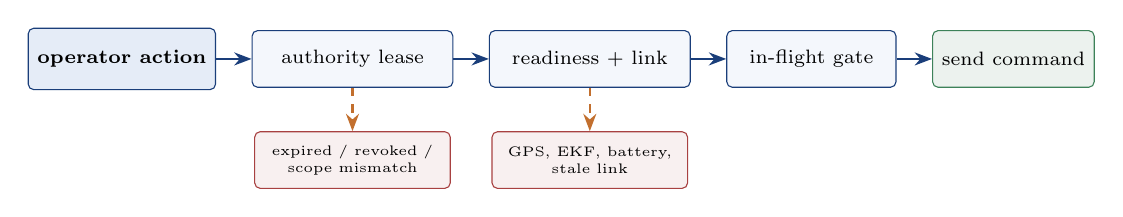
\begin{tikzpicture}[node distance=0.35cm]
  \node[strongbox,minimum width=2.3cm] (intent) {operator action};
  \node[box,right=0.45cm of intent,minimum width=2.55cm] (lease) {authority lease};
  \node[box,right=0.45cm of lease,minimum width=2.55cm] (ready) {readiness + link};
  \node[box,right=0.45cm of ready,minimum width=2.15cm] (busy) {in-flight gate};
  \node[greenbox,right=0.45cm of busy,minimum width=2.0cm] (send) {send command};
  \draw[flow] (intent) -- (lease);
  \draw[flow] (lease) -- (ready);
  \draw[flow] (ready) -- (busy);
  \draw[flow] (busy) -- (send);
  \node[redbox,below=0.55cm of lease,text width=2.25cm,font=\tiny] (deny1) {expired / revoked /\\scope mismatch};
  \node[redbox,below=0.55cm of ready,text width=2.25cm,font=\tiny] (deny2) {GPS, EKF, battery,\\stale link};
  \draw[dashflow] (lease) -- (deny1);
  \draw[dashflow] (ready) -- (deny2);
\end{tikzpicture}
\end{center}

\vspace{0.55em}
\begin{itemize}
  \item A lease binds operator, drone set, monitor/control scope, and time window.
  \item Monitor authority permits observation but does not permit flight control.
  \item Authority never overrides readiness or safety; both gates must pass.
  \item Rejection reasons and authority alerts remain visible and auditable.
\end{itemize}
\evidence{OperatorAuthorityLease; validateOperatorLease; validateFlightSafetyGate}
\end{frame}

\begin{frame}{Flight-Controller Adapter Boundary}
\footnotesize
\begin{columns}[T]
\begin{column}{0.49\textwidth}
\begin{center}
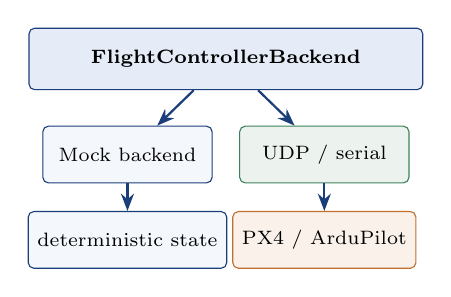
\begin{tikzpicture}[node distance=0.3cm]
  \node[strongbox,minimum width=5.0cm] (interface) {FlightControllerBackend};
  \node[box,below=0.45cm of interface,xshift=-1.25cm,minimum width=2.15cm] (mock) {Mock backend};
  \node[greenbox,below=0.45cm of interface,xshift=1.25cm,minimum width=2.15cm] (real) {UDP / serial};
  \node[box,below=0.35cm of mock,minimum width=2.15cm] (det) {deterministic state};
  \node[orangebox,below=0.35cm of real,minimum width=2.15cm] (px4) {PX4 / ArduPilot};
  \draw[flow] (interface) -- (mock);
  \draw[flow] (interface) -- (real);
  \draw[flow] (mock) -- (det);
  \draw[flow] (real) -- (px4);
\end{tikzpicture}
\end{center}
\end{column}
\begin{column}{0.47\textwidth}
\textbf{Backend contract}
\begin{itemize}
  \item forward MAVLink frames
  \item return command ACK fields
  \item expose latest telemetry
  \item read/edit parameters
  \item upload mission waypoints
\end{itemize}

\textbf{Real-link helpers}
\begin{itemize}
  \item GCS heartbeat
  \item manual-control replay
  \item neutral command after timeout
\end{itemize}
\end{column}
\end{columns}
\evidence{FlightControllerBackend; MockFlightControllerBackend; UdpFlightControllerBackend}
\end{frame}

\begin{frame}{Multi-Drone Mission Lifecycle}
\footnotesize
\begin{center}
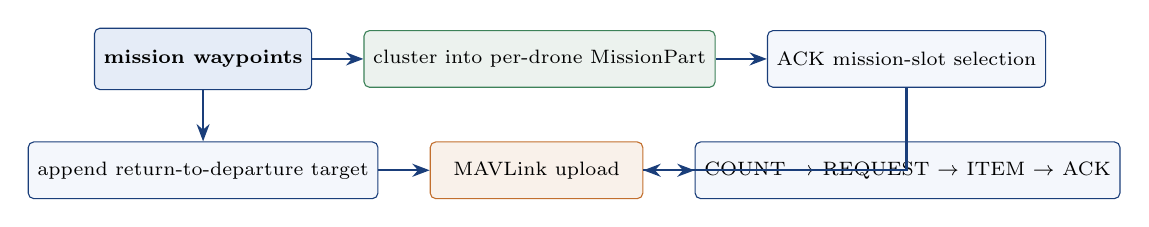
\begin{tikzpicture}[node distance=0.3cm]
  \node[strongbox,minimum width=2.5cm] (route) {mission waypoints};
  \node[greenbox,right=0.65cm of route,minimum width=3.7cm] (parts) {cluster into per-drone MissionPart};
  \node[box,right=0.65cm of parts,minimum width=3.2cm] (assign) {ACK mission-slot selection};
  \draw[flow] (route) -- (parts);
  \draw[flow] (parts) -- (assign);

  \node[box,below=0.65cm of route,minimum width=3.25cm] (return) {append return-to-departure target};
  \node[orangebox,right=0.65cm of return,minimum width=2.7cm] (upload) {MAVLink upload};
  \node[box,right=0.65cm of upload,minimum width=4.0cm] (handshake) {COUNT $\rightarrow$ REQUEST $\rightarrow$ ITEM $\rightarrow$ ACK};
  \draw[flow] (route) -- (return);
  \draw[flow] (assign) |- (upload);
  \draw[flow] (return) -- (upload);
  \draw[flow] (upload) -- (handshake);
\end{tikzpicture}
\end{center}

\vspace{0.55em}
\bluebox{Mission start is phased: arm accepted drones, take off accepted drones, then start only the mission parts that were uploaded successfully.}
\evidence{MissionPlan/MissionPart; uploadMissionPlan; executeMissionWaypoints}
\end{frame}

\begin{frame}{Mission Recovery and Persistence}
\footnotesize
\begin{columns}[T]
\begin{column}{0.49\textwidth}
\textbf{Application-level compensation}
\begin{center}
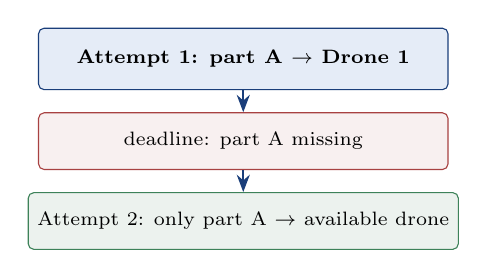
\begin{tikzpicture}[node distance=0.28cm]
  \node[strongbox,minimum width=5.2cm] (attempt1) {Attempt 1: part A $\rightarrow$ Drone 1};
  \node[redbox,below=of attempt1,minimum width=5.2cm] (missing) {deadline: part A missing};
  \node[greenbox,below=of missing,minimum width=5.2cm] (attempt2) {Attempt 2: only part A $\rightarrow$ available drone};
  \draw[flow] (attempt1) -- (missing);
  \draw[flow] (missing) -- (attempt2);
\end{tikzpicture}
\end{center}
\begin{itemize}
  \item shared \texttt{patrol\_task\_id}; fresh NDNSF request each attempt
  \item no restart of already completed mission parts
\end{itemize}
\end{column}
\begin{column}{0.47\textwidth}
\textbf{Persistent mission document}
\begin{itemize}
  \item stable plan and operator identifiers
  \item per-drone parts and waypoint order
  \item geofence/rally metadata for future expansion
  \item save, load, preview, and upload through one typed model
\end{itemize}

\bluebox{Compensation repairs missing service results; it is not autonomous in-flight route optimization.}
\end{column}
\end{columns}
\evidence{MissionProgressState; MissionPlanDocument; runPatrolCompensationTask}
\end{frame}

\begin{frame}{Setup and Inspection Services}
\footnotesize
\begin{columns}[T]
\begin{column}{0.32\textwidth}
\textbf{Parameters}
\begin{itemize}
  \item firmware, modes, completeness
  \item typed value and dry-run
  \item expected-value check
  \item read-back verification
\end{itemize}
\end{column}
\begin{column}{0.32\textwidth}
\textbf{Preflight}
\begin{itemize}
  \item named checklist items
  \item severity and blocking state
  \item operator-readable reason
  \item refresh before dangerous action
\end{itemize}
\end{column}
\begin{column}{0.32\textwidth}
\textbf{Analyze}
\begin{itemize}
  \item MAVLink message summaries
  \item active rates and last-seen state
  \item vehicle/mission snapshot
  \item inspector-oriented output
\end{itemize}
\end{column}
\end{columns}

\vspace{0.75em}
\begin{center}
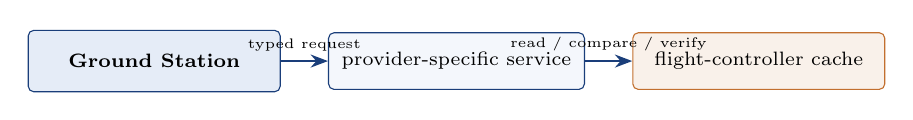
\begin{tikzpicture}[node distance=0.45cm]
  \node[strongbox,minimum width=3.2cm] (gs) {Ground Station};
  \node[box,right=0.6cm of gs,minimum width=3.25cm] (service) {provider-specific service};
  \node[orangebox,right=0.6cm of service,minimum width=3.2cm] (backend) {flight-controller cache};
  \draw[flow] (gs) -- node[above,font=\tiny] {typed request} (service);
  \draw[flow] (service) -- node[above,font=\tiny] {read / compare / verify} (backend);
\end{tikzpicture}
\end{center}
\evidence{VehicleParameterEditRequest/Result; PreflightCheckItem; UavAnalyzeSnapshot}
\end{frame}

\begin{frame}{Live Video: Control and Data Are Separate}
\footnotesize
\begin{center}
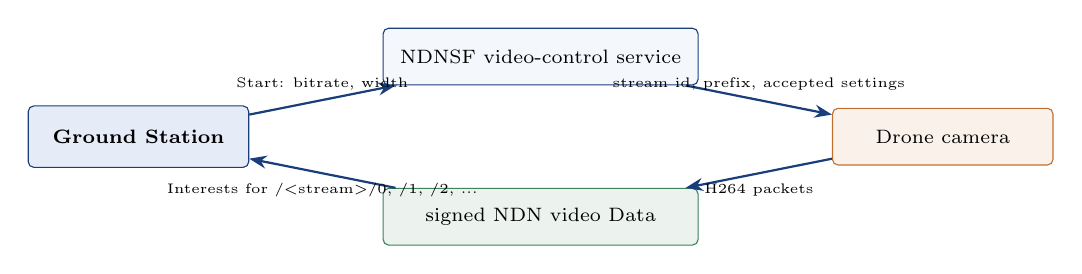
\begin{tikzpicture}[node distance=0.45cm]
  \node[strongbox,minimum width=2.8cm] (gs) {Ground Station};
  \node[orangebox,right=7.4cm of gs,minimum width=2.8cm] (drone) {Drone camera};
  \node[box,above=0.65cm of $(gs)!0.5!(drone)$,minimum width=4.0cm] (control) {NDNSF video-control service};
  \node[greenbox,below=0.65cm of $(gs)!0.5!(drone)$,minimum width=4.0cm] (data) {signed NDN video Data};
  \draw[flow] (gs) -- node[above,font=\tiny] {Start: bitrate, width} (control);
  \draw[flow] (control) -- node[above,font=\tiny] {stream id, prefix, accepted settings} (drone);
  \draw[backflow] (gs) -- node[below,font=\tiny] {Interests for /<stream>/0, /1, /2, ...} (data);
  \draw[backflow] (data) -- node[below,font=\tiny] {H264 packets} (drone);
\end{tikzpicture}
\end{center}

\vspace{0.75em}
\begin{itemize}
  \item The service response starts or stops a session; it does not carry the video stream.
  \item Packet names are predictable and monotonically increasing within a stream.
  \item Stop is idempotent; late Interests and packets from the stopped session are ignored.
\end{itemize}
\evidence{VideoPublisher::start/stop; startVideoAttempt; README Video Streaming Design}
\end{frame}

\begin{frame}{Stream Packet and Session Model}
\footnotesize
\begin{columns}[T]
\begin{column}{0.52\textwidth}
\begin{center}
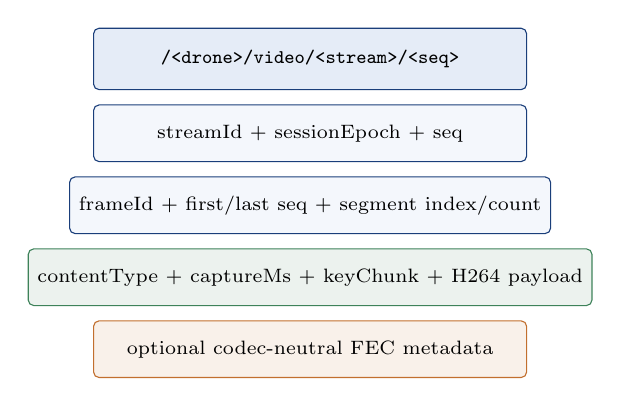
\begin{tikzpicture}[node distance=0.18cm]
  \node[strongbox,minimum width=5.5cm] (name) {\texttt{/<drone>/video/<stream>/<seq>}};
  \node[box,below=of name,minimum width=5.5cm] (session) {streamId + sessionEpoch + seq};
  \node[box,below=of session,minimum width=5.5cm] (frame) {frameId + first/last seq + segment index/count};
  \node[greenbox,below=of frame,minimum width=5.5cm] (payload) {contentType + captureMs + keyChunk + H264 payload};
  \node[orangebox,below=of payload,minimum width=5.5cm] (fec) {optional codec-neutral FEC metadata};
\end{tikzpicture}
\end{center}
\end{column}
\begin{column}{0.44\textwidth}
\textbf{Consumer guards}
\begin{itemize}
  \item reject an old stream id or session epoch
  \item suppress duplicate packet sequence numbers
  \item reorder chunks before decoder input
  \item skip a late missing delta chunk to keep playback live
\end{itemize}

\bluebox{\texttt{VideoPacket} maps to core \texttt{StreamChunk} semantics without changing the existing UAV wire format.}
\end{column}
\end{columns}
\evidence{Stream.hpp; VideoPacket; videoPacketToStreamChunk; isCurrentVideoSessionPacket}
\end{frame}

\begin{frame}{Adaptive Receiver Control Loop}
\footnotesize
\begin{center}
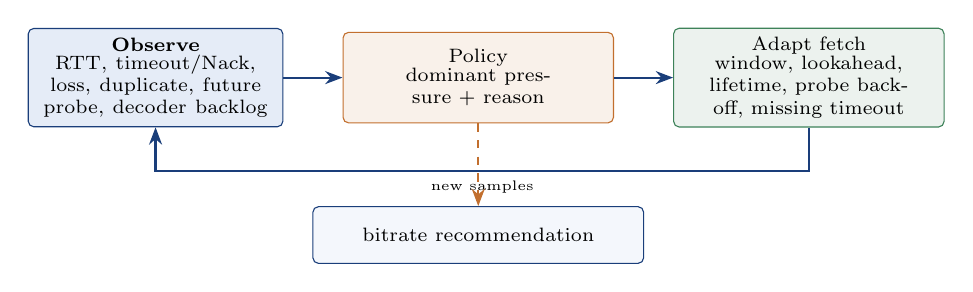
\begin{tikzpicture}[node distance=0.45cm]
  \node[strongbox,text width=3.0cm,minimum height=1.15cm] (observe) {
    Observe\\[-0.15em]
    \normalfont RTT, timeout/Nack, loss, duplicate, future probe, decoder backlog
  };
  \node[orangebox,right=0.75cm of observe,text width=3.2cm,minimum height=1.15cm] (policy) {
    Policy\\[-0.15em]
    \normalfont dominant pressure + reason
  };
  \node[greenbox,right=0.75cm of policy,text width=3.2cm,minimum height=1.15cm] (adapt) {
    Adapt fetch\\[-0.15em]
    \normalfont window, lookahead, lifetime, probe backoff, missing timeout
  };
  \draw[flow] (observe) -- (policy);
  \draw[flow] (policy) -- (adapt);
  \draw[flow] (adapt.south) -- ++(0,-0.55cm) -| node[below,pos=0.25,font=\tiny] {new samples} (observe.south);

  \node[box,below=1.05cm of policy,minimum width=4.2cm] (advice) {bitrate recommendation};
  \draw[dashflow] (policy) -- (advice);
\end{tikzpicture}
\end{center}

\vspace{0.35em}
\bluebox{Fetch adaptation is automatic. A producer bitrate change is explicit: Stop the old session, then Start a coherent new session with the requested bitrate.}
\evidence{VideoAdaptivePolicyInput/Decision; requestVideoLane; restartVideoWithBitrateAfterStop}
\end{frame}

\begin{frame}{One-Loss XOR Forward Error Correction}
\footnotesize
\begin{columns}[T]
\begin{column}{0.62\textwidth}
\begin{center}
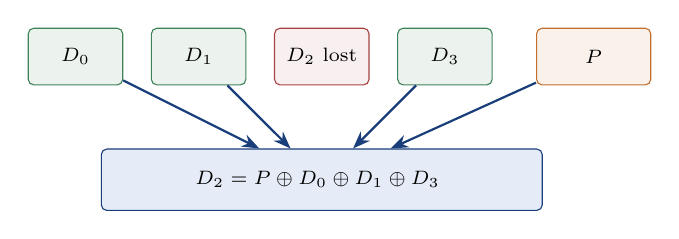
\begin{tikzpicture}[node distance=0.35cm]
  \node[greenbox,minimum width=1.2cm] (d0) {$D_0$};
  \node[greenbox,right=of d0,minimum width=1.2cm] (d1) {$D_1$};
  \node[redbox,right=of d1,minimum width=1.2cm] (d2) {$D_2$ lost};
  \node[greenbox,right=of d2,minimum width=1.2cm] (d3) {$D_3$};
  \node[orangebox,right=0.55cm of d3,minimum width=1.45cm] (p) {$P$};
  \node[strongbox,below=0.8cm of d2,minimum width=5.6cm] (recover) {
    $D_2 = P \oplus D_0 \oplus D_1 \oplus D_3$
  };
  \draw[flow] (d0) -- (recover);
  \draw[flow] (d1) -- (recover);
  \draw[flow] (d3) -- (recover);
  \draw[flow] (p) -- (recover);
\end{tikzpicture}
\end{center}
\end{column}
\begin{column}{0.34\textwidth}
\textbf{Current behavior}
\begin{itemize}
  \item one parity shard per frame by default
  \item original lengths carried in metadata
  \item recover before decoder insertion
  \item more than one missing data shard is not recoverable
\end{itemize}
\end{column}
\end{columns}

\vspace{0.55em}
\bluebox{FEC reduces retransmission delay for a single hole; reorder and stale-frame skipping preserve liveness when recovery is impossible.}
\evidence{VideoPublisher::publishCurrentFrame; processFecChunk; attemptAndRecoverFrame}
\end{frame}

\begin{frame}{Recording Is a Named Object, Not a Live Stream}
\footnotesize
\begin{center}
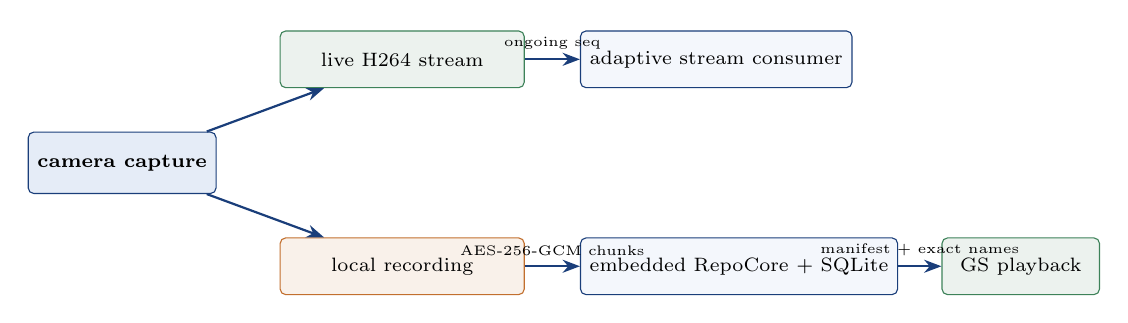
\begin{tikzpicture}[node distance=0.35cm]
  \node[strongbox,minimum width=2.35cm] (camera) {camera capture};
  \node[greenbox,above right=0.55cm and 0.8cm of camera,minimum width=3.1cm] (live) {live H264 stream};
  \node[orangebox,below right=0.55cm and 0.8cm of camera,minimum width=3.1cm] (record) {local recording};
  \node[box,right=0.7cm of live,minimum width=3.0cm] (consumer) {adaptive stream consumer};
  \node[box,right=0.7cm of record,minimum width=3.0cm] (repo) {embedded RepoCore + SQLite};
  \node[greenbox,right=0.55cm of repo,minimum width=2.0cm] (playback) {GS playback};
  \draw[flow] (camera) -- (live);
  \draw[flow] (camera) -- (record);
  \draw[flow] (live) -- node[above,font=\tiny] {ongoing seq} (consumer);
  \draw[flow] (record) -- node[above,font=\tiny] {AES-256-GCM chunks} (repo);
  \draw[flow] (repo) -- node[above,font=\tiny] {manifest + exact names} (playback);
\end{tikzpicture}
\end{center}

\vspace{0.65em}
\begin{itemize}
  \item Capture, recording, and viewing have independent lifecycles.
  \item The manifest and catalog discover durable chunks under publisher-owned names.
  \item Playback fetches and decrypts named chunks; it does not continue the live stream session.
\end{itemize}
\evidence{VideoPublisher recording path; RepoCore; Ground Station recording playback}
\end{frame}

\begin{frame}{Ground-Station Object Detection Callback}
\footnotesize
\begin{center}
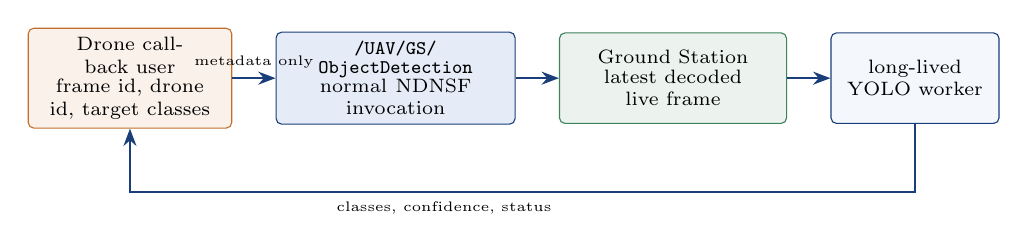
\begin{tikzpicture}[node distance=0.55cm]
  \node[orangebox,text width=2.35cm,minimum height=1.15cm] (drone) {
    Drone callback user\\[-0.1em]
    \normalfont frame id, drone id, target classes
  };
  \node[strongbox,right=0.55cm of drone,text width=2.8cm,minimum height=1.15cm] (service) {
    \texttt{/UAV/GS/}\\[-0.15em]\texttt{ObjectDetection}\\[-0.1em]
    \normalfont normal NDNSF invocation
  };
  \node[greenbox,right=0.55cm of service,text width=2.65cm,minimum height=1.15cm] (frame) {
    Ground Station\\[-0.1em]
    \normalfont latest decoded live frame
  };
  \node[box,right=0.55cm of frame,text width=1.9cm,minimum height=1.15cm] (yolo) {
    long-lived\\YOLO worker
  };
  \draw[flow] (drone) -- node[above,font=\tiny] {metadata only} (service);
  \draw[flow] (service) -- (frame);
  \draw[flow] (frame) -- (yolo);
  \draw[backflow] (drone.south) -- ++(0,-0.8cm) -| node[below,pos=0.2,font=\tiny] {classes, confidence, status} (yolo.south);
\end{tikzpicture}
\end{center}

\vspace{0.7em}
\bluebox{Roles can reverse: a drone is normally a provider, but it can consume a heavier service from the ground station. Image bytes are reused locally and are not inserted into the service request.}
\evidence{installObjectDetectionService; startObjectDetectionLoop; yolo\_detect\_worker.py}
\end{frame}

\begin{frame}{One Runtime, GUI or Headless}
\footnotesize
\begin{columns}[T]
\begin{column}{0.47\textwidth}
\begin{center}
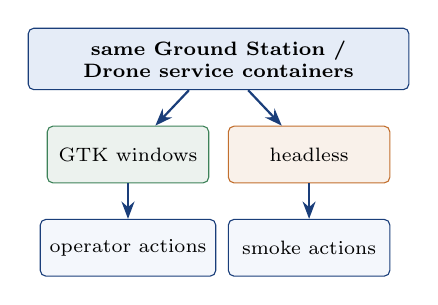
\begin{tikzpicture}[node distance=0.28cm]
  \node[strongbox,text width=4.6cm] (runtime) {same Ground Station / Drone service containers};
  \node[greenbox,below=0.45cm of runtime,xshift=-1.15cm,minimum width=2.05cm] (gui) {GTK windows};
  \node[orangebox,below=0.45cm of runtime,xshift=1.15cm,minimum width=2.05cm] (headless) {headless};
  \node[box,below=0.45cm of gui,minimum width=2.05cm] (human) {operator actions};
  \node[box,below=0.45cm of headless,minimum width=2.05cm] (auto) {smoke actions};
  \draw[flow] (runtime) -- (gui);
  \draw[flow] (runtime) -- (headless);
  \draw[flow] (gui) -- (human);
  \draw[flow] (headless) -- (auto);
\end{tikzpicture}
\end{center}
\end{column}
\begin{column}{0.49\textwidth}
\textbf{Validation layers}
\begin{itemize}
  \item C++ protocol/state unit tests
  \item deployment and config quick smoke
  \item MiniNDN multi-node service tests
  \item PX4 SITL + jMAVSim command/mission tests
  \item GUI smoke under Xvfb
\end{itemize}

\textbf{Default MiniNDN placement}
\begin{itemize}
  \item Controller + GS: Memphis
  \item Drone A: UCLA
  \item Drone B: WUSTL
\end{itemize}
\end{column}
\end{columns}
\evidence{MiniNDN UAV launcher; UAV protocol/state unit tests}
\end{frame}

\begin{frame}{Implemented Foundation and Current Boundary}
\footnotesize
\begin{columns}[T]
\begin{column}{0.49\textwidth}
\textbf{Implemented foundation}
\begin{itemize}
  \item named, permission-controlled UAV services
  \item Targeted command path and typed control state
  \item operator authority and safety gates
  \item multi-drone mission assignment and compensation
  \item adaptive H264 delivery with session guards and XOR FEC
  \item encrypted recording discovery and playback
\end{itemize}
\end{column}
\begin{column}{0.47\textwidth}
\textbf{Not yet a production ground station}
\begin{itemize}
  \item complete calibration and firmware setup
  \item full survey/geofence/altitude-profile editing
  \item hardened lost-link and autopilot fail-safe policy
  \item long-duration outdoor and hardware-breadth evidence
  \item certified operator workflow and safety assurance
\end{itemize}
\end{column}
\end{columns}

\vspace{0.65em}
\bluebox{Next: use repeated real-device campaigns to harden safety and recovery, while moving only genuinely app-neutral mechanisms back into NDNSF Core.}
\evidence{NDNSF-UAV-APP/README.md: Current Boundary and Comparison With QGroundControl}
\end{frame}

\end{document}
